%!TEX root = ../toolhinweise.tex

\section{Nutzung von YAKINDU SCT}
\label{sec:yakindu}

In diesem Abschnitt werden ergänzend zur Vorstellung der Syntax-Besonderheiten in \autoref{sec:syntax} einige Hinweise zur Nutzung von YAKINDU SCT gegeben.

Eine detaillierte Erläuterung zu YAKINDU SCT findet sich unter \url{https://www.itemis.com/en/yakindu/state-machine/documentation/user-guide/edit_editing_statecharts}.

\enlargethispage{1\baselineskip}




%%%%%%%%%%%%%%%%%%%%%%%%%%%%%%%%%%%%%%%%%%%%%%%%%%%%%%%%%%%%%%%%%%%%%%%%%%%%%%%%%%%%%%%%%%%%




\subsection{Nutzung von Versionskontrollsystemen}

Ein Statechart in YAKINDU SCT ist in einer einzigen .sct-Datei gespeichert. 
Die .sct-Dateien können \emph{nicht} gemergt werden. 
Bei der Verwendung eines Versionskontrollsystems (z.B. Git) ist also auf die Vermeidung von Konflikten zu achten.

Wenn parallel auf verschiedenen Geräten an verschiedenen Statechart-Features gearbeitet wird, besteht die Möglichkeit, eine der .sct-Dateien (und die dazugehörige .sgen-Datei) umzubenennen. 
Die Codegenerierung ist so weiterhin möglich. 
Zum Zusammenführen der .sct-Dateien ist es in YAKINDU SCT möglich Diagrammelemente zwischen diesen Dateien zu kopieren.




%%%%%%%%%%%%%%%%%%%%%%%%%%%%%%%%%%%%%%%%%%%%%%%%%%%%%%%%%%%%%%%%%%%%%%%%%%%%%%%%%%%%%%%%%%%%




\subsection{Modellierung von Statecharts}

\begin{figure}[t]
	\centering
	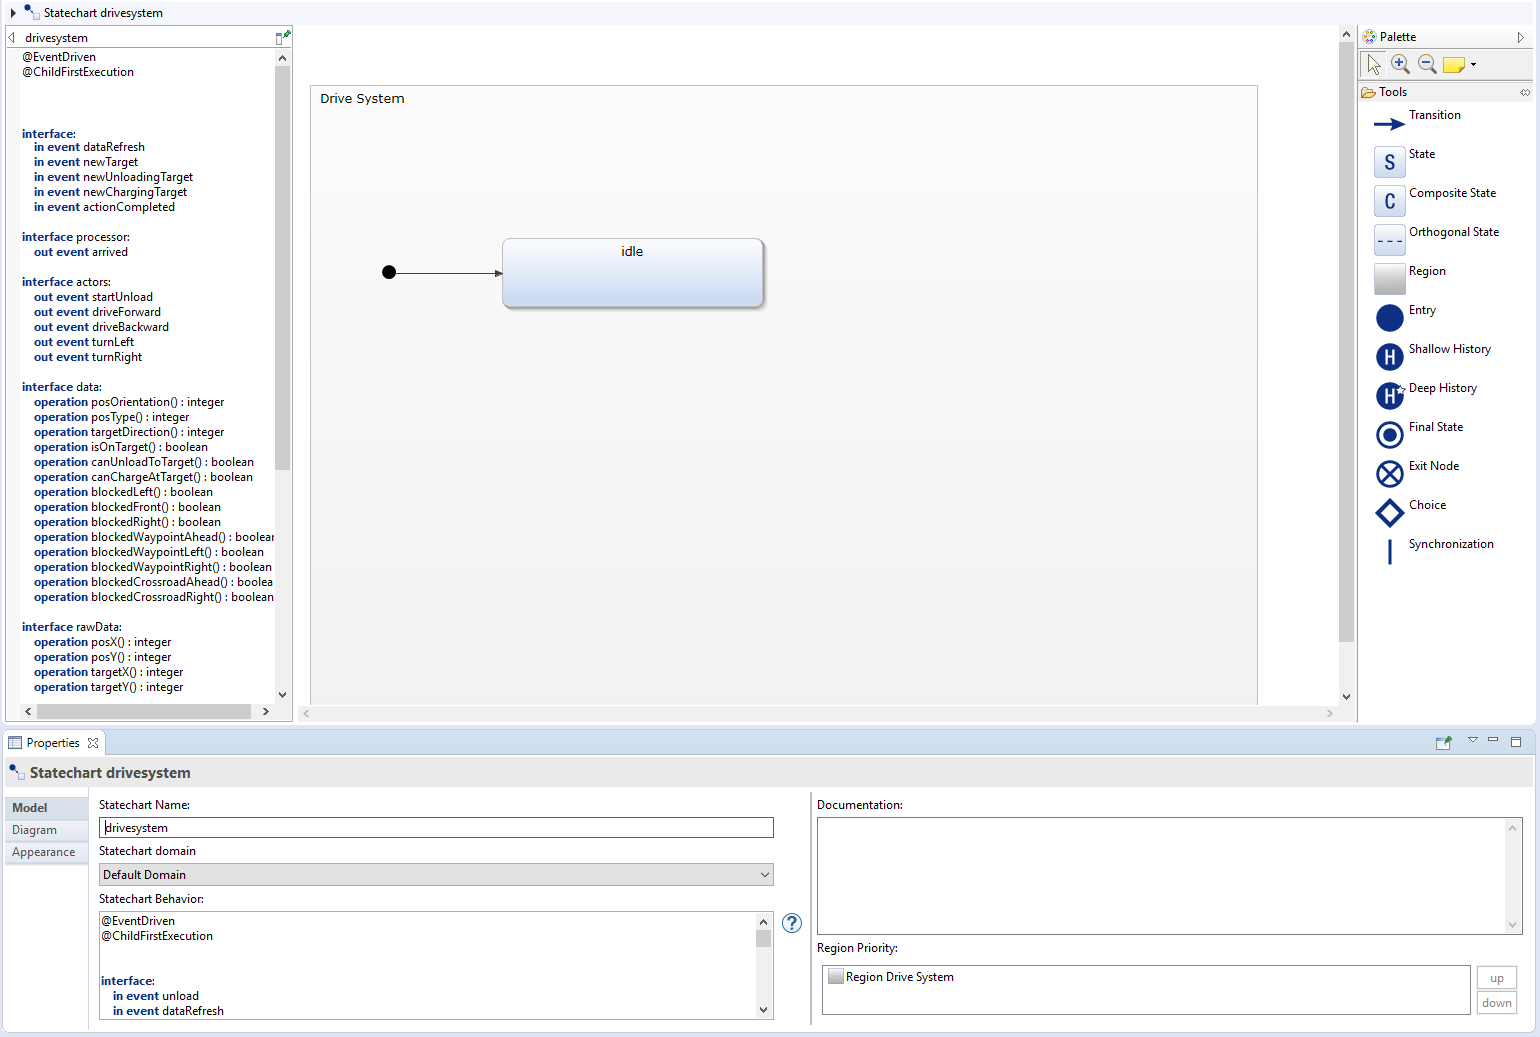
\includegraphics[width=1\textwidth]{yakindu_fenster}
	\caption{Die Modellierungsansicht in YAKINDU SCT}
	\label{fig:yakindu_ui}
\end{figure}

Das im \docProjectTitle{} zu modellierende Statechart befindet sich im Ordner \texttt{model}. 
Per Doppelklick auf die entsprechende Datei \texttt{infinitewarehouse\_drivesystem.sct} (oder auf eine andere .sct-Datei) öffnet sich die Modellierungsansicht.

Sollte sich die Modellierungansicht nicht wie erwartet öffnen, muss die aktuell gewählte Perspektive überprüft werden (kleine Icons oben rechts). 
Hier ist \enquote{SC Modeling} auszuwählen. 


\subsubsection{Überblick}
 
Die Modellierungsansicht (siehe \autoref{fig:yakindu_ui}) ist wie folgt strukturiert:

\begin{itemize}
	\setlength\topsep{-1em}
	\setlength\itemsep{-0.5em}
	\item In der Bildschirmmitte befindet sich das eigentliche Statechart-Diagramm.
	\item Auf der linken Seite befindet sich der Definitionsbereich des Statecharts, der dem Klassendiagramm aus dem Entwurfsdokument (siehe Abbildung 5 dort) entspricht. 
	Dieser Definitionsbereich darf nicht verändert werden und dient lediglich als Referenz. 
	Interne Ereignisse und Variablen (gekennzeichnet durch das Schlüsselwort \enquote{internal}) dürfen allerdings ergänzt werden.
	\item Auf der rechten Seite befindet sich die Palette mit den Diagrammelementen, die zur Modellierung genutzt werden können. 
	Besonders wichtig sind hierbei die Elemente \enquote{State} (um einen neuen Zustand anzulegen), \enquote{Transition} (um eine Transition zwischen zwei Elementen einzufügen) und \enquote{Choice} (um eine Entscheidung zu definieren).
	\item Im unteren Bereich befindet sich das \enquote{Properties}-Fenster, in dem Eigenschaften des aktuell ausgewählten Elements zu finden sind.
\end{itemize}


\enlargethispage{2\baselineskip}

\subsubsection{Syntax und Konventionen}

Für das Statechart ist die aus der Vorlesung bekannte Syntax zu verwenden.

Zusätzlich gelten einige Konventionen bei der Benennung der Zustände und Regionen. 
Das sollte dem Framework ermöglichen den aktuellen Zustand des Statecharts anzuzeigen:
\begin{itemize}
	\setlength\topsep{-1em}
	\setlength\itemsep{-0.5em}
	\item Die äußerste Region muss \enquote{\texttt{Drive System}} heißen.
	\item Wenn bei der Modellierung (abgesehen von der äußersten Region) weitere Regionen verwendet werden, müssen diese entweder unbenannt sein oder deren Namen müssen mit einem Unterstrich (\enquote{\texttt{\_}}) beginnen. 
	Die Regionnamen dürfen keine Leerzeichen und keine weiteren Unterstriche enthalten.
	\item In Zustandsnamen dürfen keine Unterstriche benutzt werden.
\end{itemize}



\subsubsection{Modellierung von Reaktionen}

Mittels Doppelklick auf den unteren Bereich eines Zustandes öffnet sich ein Textfeld, in dem lokale Reaktionen (z.B. mit \enquote{entry} oder \enquote{exit} als Trigger) spezifiziert werden können.
Mittels Doppelklick auf eine Transition öffnet sich ein Textfeld, in dem auch eine Reaktion spezifiziert werden kann. 

Die Trigger einer Reaktion können jeweils direkt angegeben werden.
Nach den Triggern können Guards in eckigen Klammern definiert werden.
Innerhalb eines Guards können Operationen und Variablen aus dem Definitionsbereich verwendet werden. 

\begin{center}
	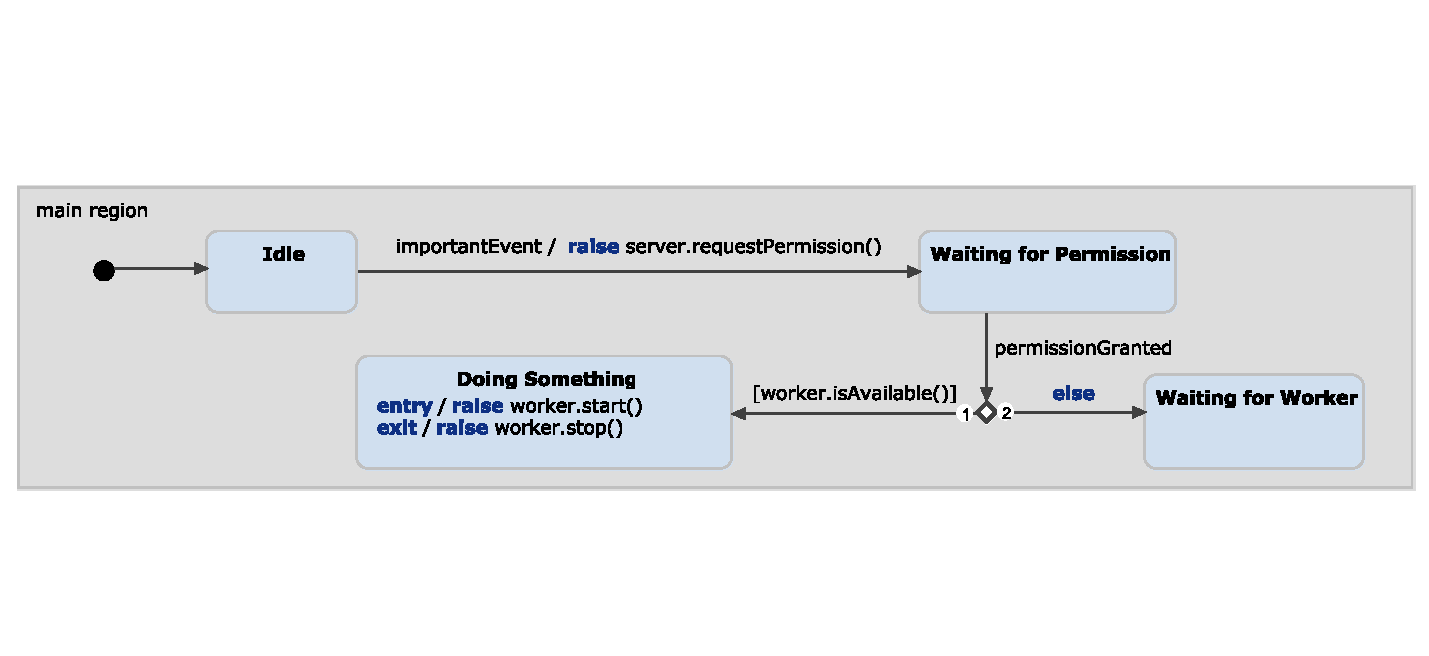
\includegraphics[width=\textwidth]{yakindu_reaktionen}	
\end{center}

Die Effekte sind durch ein \enquote{\texttt{/}} von Triggern und Guards zu trennen. 
Hier können unter anderem ausgehende oder interne Ereignisse genutzt werden, die mit dem Schlüsselwort \enquote{raise} eingeleitet werden.
 
Aus einer Entscheidung oder einem Zustand ausgehende Transitionen sind jeweils nummeriert. 
Die Zahlen geben dabei die Reihenfolge an, in der die Transitionen ausgewertet werden.
Es wird also zuerst die Transition mit der Priorität~1 ausgewertet. 
Wenn die Transition eine Bedingung hat und diese Bedingung wahr ist, werden die Effekte dieser Transition ausgeführt, ansonsten wird die Transition mit der nächsthöchsten Priorität ausgewertet.
Die Prioritäten der ausgehenden Transitionen können im \enquote{Properties}-Fenster einer Entscheidung oder eines Zustandes angepasst werden.


\subsubsection{Subdiagramme}
Um das Statechart übersichtlich zu halten, ist es möglich Subdiagramme anzulegen. 
Dazu kann ein beliebiger Zustand rechts angeklickt und dann \enquote{Create Subdiagramm} ausgewählt werden, um den Zustand mit einem Subdiagramm zu versehen. 
Solcher Zustand ist dann mit einem kleinen Icon unten rechts markiert. 
%Dieses Icon kann angeklickt werden, um das Subdiagramm zu öffnen.
Statt eines Zustandes mit Subdiagramm kann auch ein hierarchischer Zustand genutzt werden.

Ein Zustand mit Subdiagramm bzw. ein hierarchischer Zustand muss genau eine ausgehende Transition ohne Trigger haben. 

\begin{center}
	\raisebox{-\height}{
		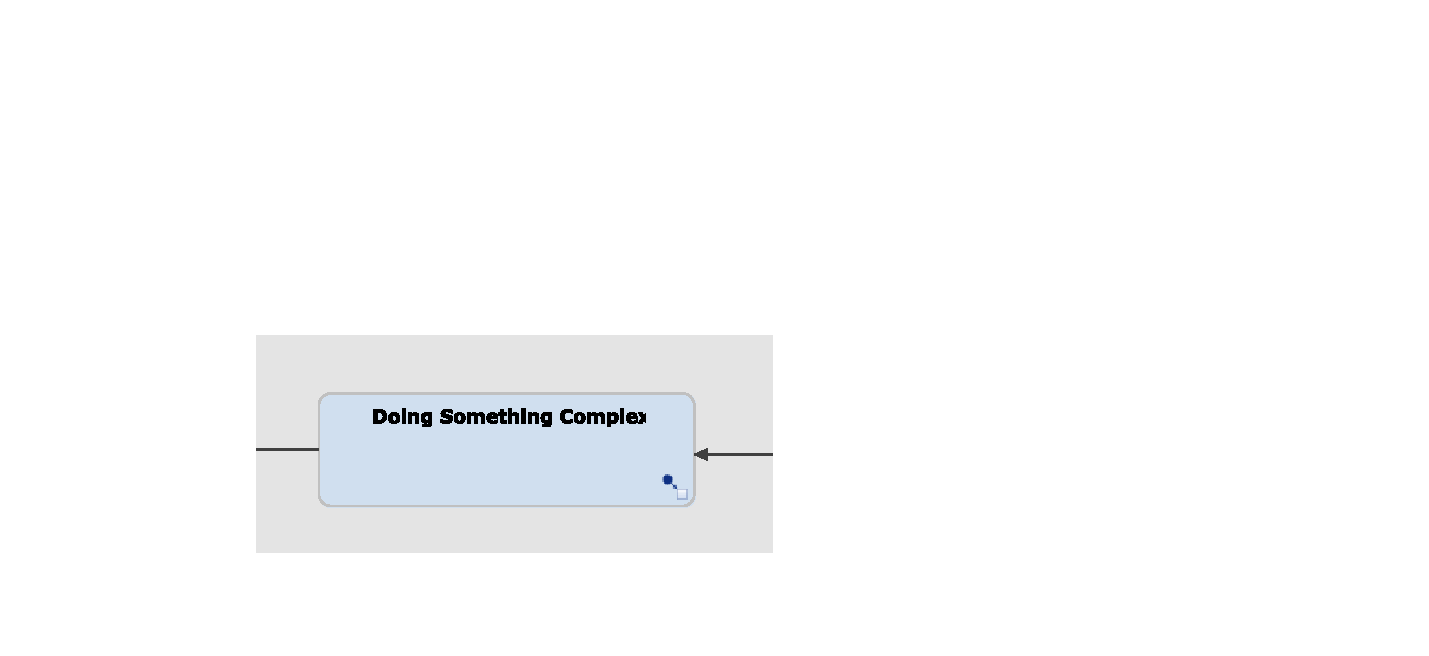
\includegraphics[scale=0.6]{yakindu_subdiagram_extern}	
	}
	~~~~~~~~~~~
	\raisebox{-\height}{
		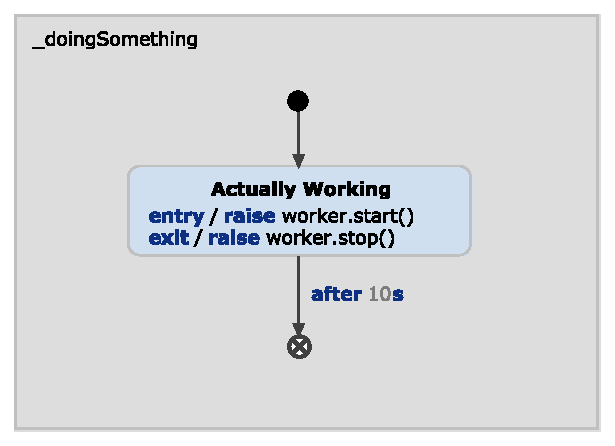
\includegraphics[scale=0.6]{yakindu_subdiagram_intern}	
	}
\end{center}
 
Durch einen Klick auf das Icon in der rechten unteren Ecke eines solchen Zustandes wird das Subdiagramm in einem neuen Tab geöffnet. 
Hier muss zuerst eine neue Region angelegt werden. 
Innerhalb dieser Region kann nun frei modelliert werden (insbesondere können mehrere Subdiagramme ineinander geschachtelt werden).
Dabei muss beachtet werden, dass es innerhalb der angelegten Region ein \enquote{Entry} sowie einen \enquote{Exit Node} geben muss (nicht zu verwechseln mit dem \enquote{Final State}). 
Nachdem das Subdiagramm diesen \enquote{Exit Node} erreicht hat, wird die Behandlung des äußeren Diagramms entlang der triggerlosen Kante fortgesetzt.




%%%%%%%%%%%%%%%%%%%%%%%%%%%%%%%%%%%%%%%%%%%%%%%%%%%%%%%%%%%%%%%%%%%%%%%%%%%%%%%%%%%%%%%%%%%%
 



\subsection{Simulation}

Das Simulationsfeature von YAKINDU SCT ermöglicht ein manuelles Simulieren und Testen des Statecharts. 
Man startet die Simulation für die .sct-Datei durch einen Klick auf den \enquote{Run}-Button.

Der Modellierungsbereich wird während einer Simulation durch eine Ansicht ersetzt, in der das Statechart nicht mehr bearbeitet werden kann, aber der aktuelle Zustand bzw. die aktuellen Zustände des Statecharts gelb markiert sind.
Im Simulationsmenü (Tab \enquote{Simulation} rechts) können Trigger ausgelöst sowie die Rückgabewerte von Operationen gesetzt werden.

Eine laufende Simulation kann durch einen Klick auf das rote Rechteck (\enquote{Stop}-Symbol) oben im Simulationsmenü beendet werden.




%%%%%%%%%%%%%%%%%%%%%%%%%%%%%%%%%%%%%%%%%%%%%%%%%%%%%%%%%%%%%%%%%%%%%%%%%%%%%%%%%%%%%%%%%%%%
 



\subsection{Codegenerierung}

Neben der internen Simulation bietet YAKINDU SCT die Möglichkeit, Code aus einem State\-chart zu generieren. 
Dies ermöglicht dann das Einbinden dieses Codes in eine eigene Simulationsumgebung (z.B. in den im \autoref{sec:framework} beschriebenen Validierungsframework).

Zur Codegenerierung muss auf die mitgelieferte Konfigurationsdatei \texttt{infinitewarehouse\_drivesystem.sgen} rechts geklickt und \enquote{Generate Code Artifacts} ausgewählt werden.
Nach der Erfolgsmeldung im Konsolenfenster befindet sich der generierte Quelltext im Ordner \texttt{src-gen}. 
%Die Roboter verhalten sich dann im Simulator entsprechend dem zuletzt generierten Code.

\enlargethispage{1\baselineskip}




%%%%%%%%%%%%%%%%%%%%%%%%%%%%%%%%%%%%%%%%%%%%%%%%%%%%%%%%%%%%%%%%%%%%%%%%%%%%%%%%%%%%%%%%%%%%
 


 

\subsection{Bekannte Probleme}

In seltenen Fällen reagiert die Modellierungsansicht von YAKINDU SCT nicht mehr auf alle Mausklicks und Tastendrücke (z.B. auf die \enquote{Entf}-Taste).
Um dies zu beheben, genügt es die .sct-Datei zu schließen und erneut zu öffnen.